\newpage
\section{Utente Non Registrato}

	\subsection{Homepage}
		La schermata principale dell'applicazione appare come mostrato nella figura sottostante ed è visibile a qualsiasi tipologia di utente.
		
		\label{Homepage}
		\begin{figure}[H]
			\centering
			\fbox{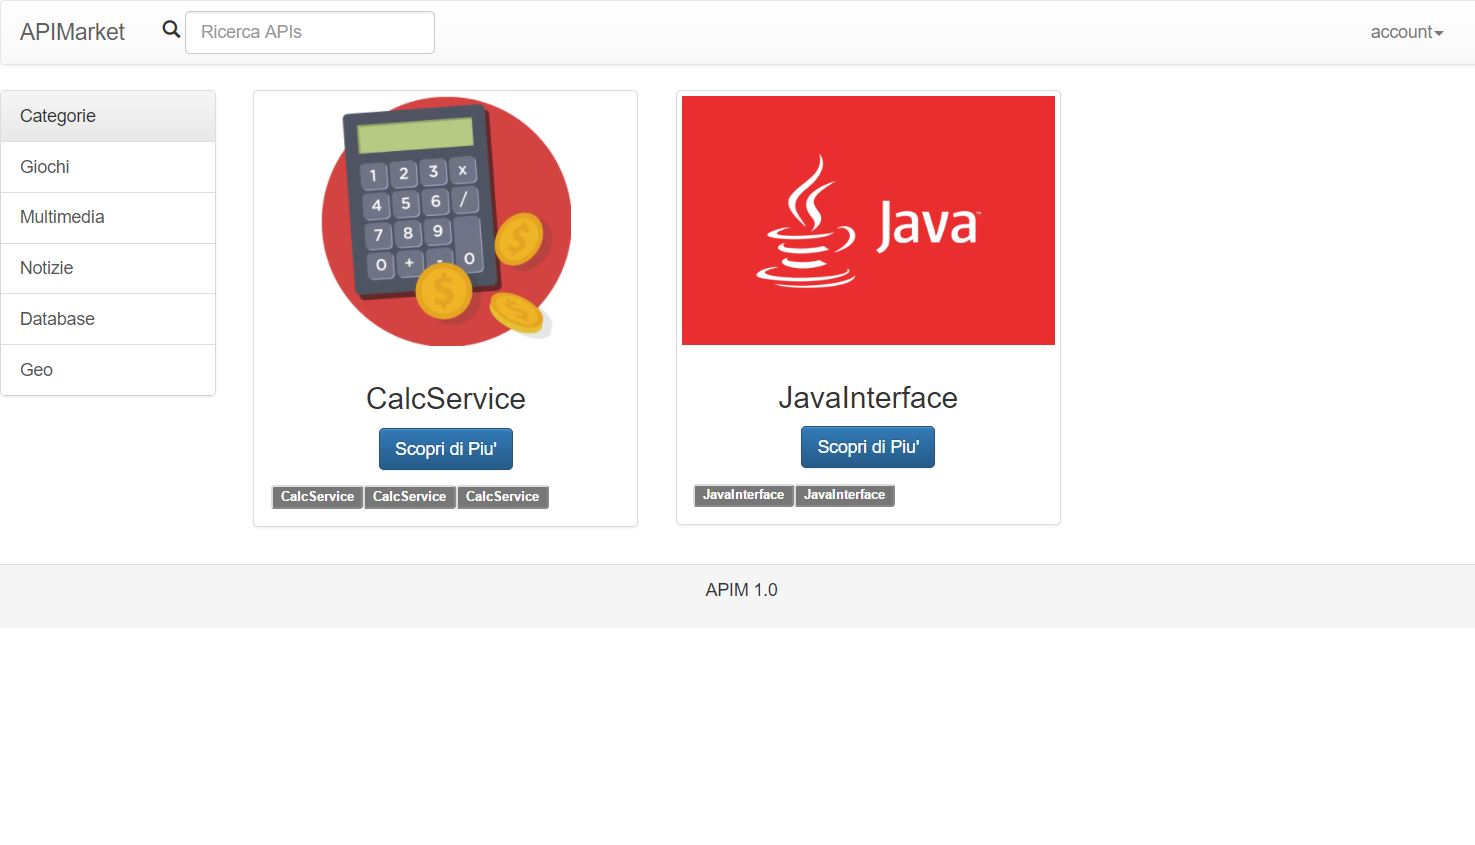
\includegraphics[scale=0.29]{img/APIM_home.JPG}}
			\caption{Homepage}
		\end{figure}
		
		Dalla schermata principale sono possibili le principali funzionalità dell'utente non autenticato. L'utente può registrarsi e autenticarsi tramite il menu in alto a destra, mentre a sinistra può sfogliare le varie categorie di API esposte nel market. Tramite la barra di ricerca, posta alla destra del logo del market, può effettuare una ricerca tramite keyword. Nella parte centrale dell'immagine sono disponibili le ultime otto API inserite all'interno dell'API Market.
		In fondo alla pagina è presente il footer, che contiene alcune informazioni sull'API Market.
		Come è possibile notare nella Figura 1, per la homepage, come per il resto della piattaforma è stato scelto un layout minimale e semplice per renderlo di facile utilizzo a diverse tipologie di utente.

	\subsection{Registrazione}
	Per poter usufruire delle funzionalità complete dell'API Market, quali acquisto e vendita di API, è necessario registrarsi. \MakeUppercase{è} possibile registrarsi alla piattaforma premendo il pulsante preposto nella barra superiore. La schermata che apparirà all'utente sarà la seguente:
	
	\label{Registrazione}
	\begin{figure}[H]
		\centering
		\fbox{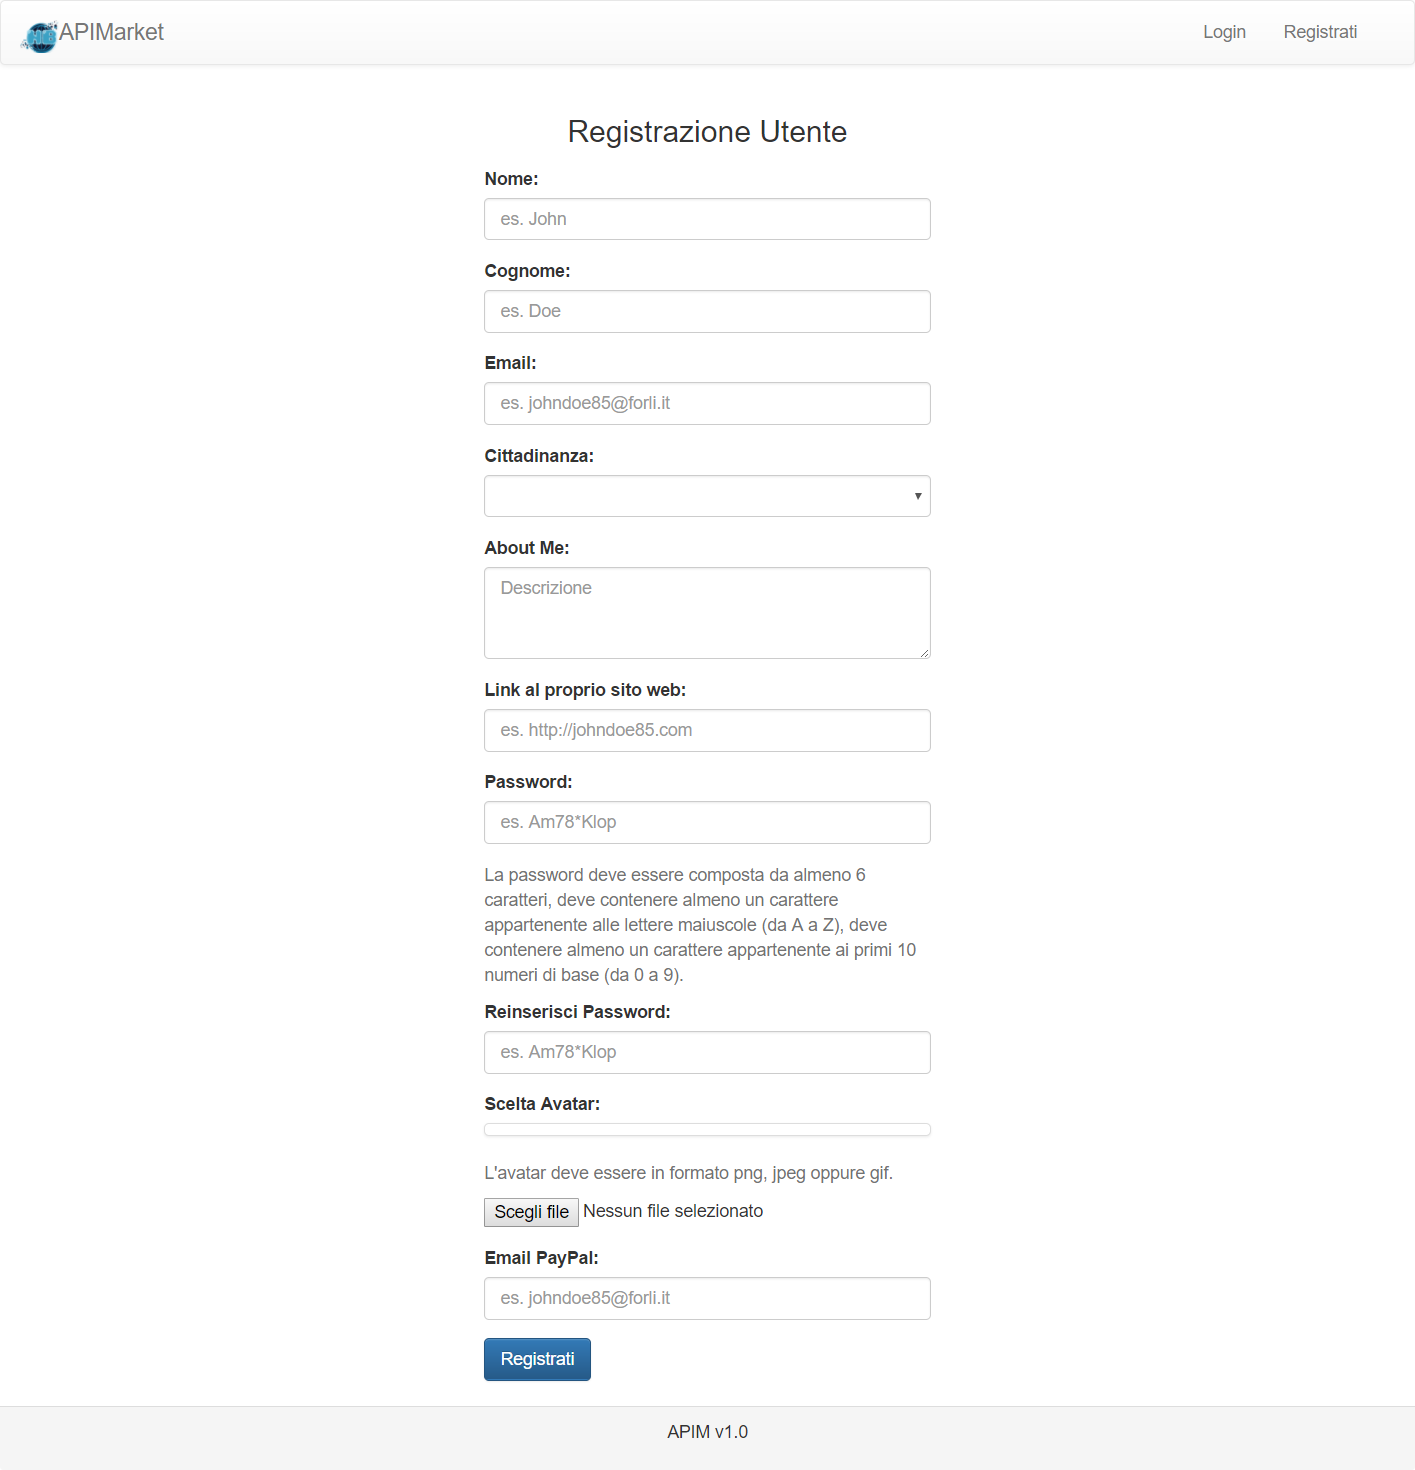
\includegraphics[scale=0.31]{img/APIM_registrazione.JPG}}
		\caption{Registrazione}
	\end{figure}
	
	Un utente per registrarsi dovrà compilare correttamente i seguenti campi, che sono obbligatori:
	\begin{itemize}
		\item Nome;
		\item Cognome;
		\item Username desiderato;
		\item Stato di residenza;
		\item Indirizzo e-mail;
		\item Password desiderata;
		\item Conferma password.
	\end{itemize}
	
	Qualora questi dati non fossero presenti o corretti, il sistema segnala un errore all'atto di registrazione e l'utente deve inserire dei parametri validi nei campi indicati. Sono presenti inoltre dei campi opzionali, destinati all'utente che vuole essere anche sviluppatore:
	
	\begin{itemize}
		\item Descrizione personale;
		\item Immagine personale;
		\item Email PayPal.
	\end{itemize}
	
	Questi campi, seppur non obbligatori, bloccano la registrazione qualora il loro inserimento non fosse effettuato in modo corretto. Si prega di prestare attenzione ai requisiti visualizzati nella schermata di registrazione.
	
	\subsection{Login}
	
	Tramite la barra superiore, vicino al pulsante di registrazione è possibile effettuare il login. La schermata di login può essere visualizzata a partire da ogni pagina non autenticata, selezionando l'apposita voce.
	Il login può essere effettuato da un utente precedentemente registrato e dalla schermata di login è possibile autenticarsi nella piattaforma per poter svolgere le funzionalità preposte agli utenti registrati. 
	
	\label{Login}
	\begin{figure}[H]
		\centering
		\fbox{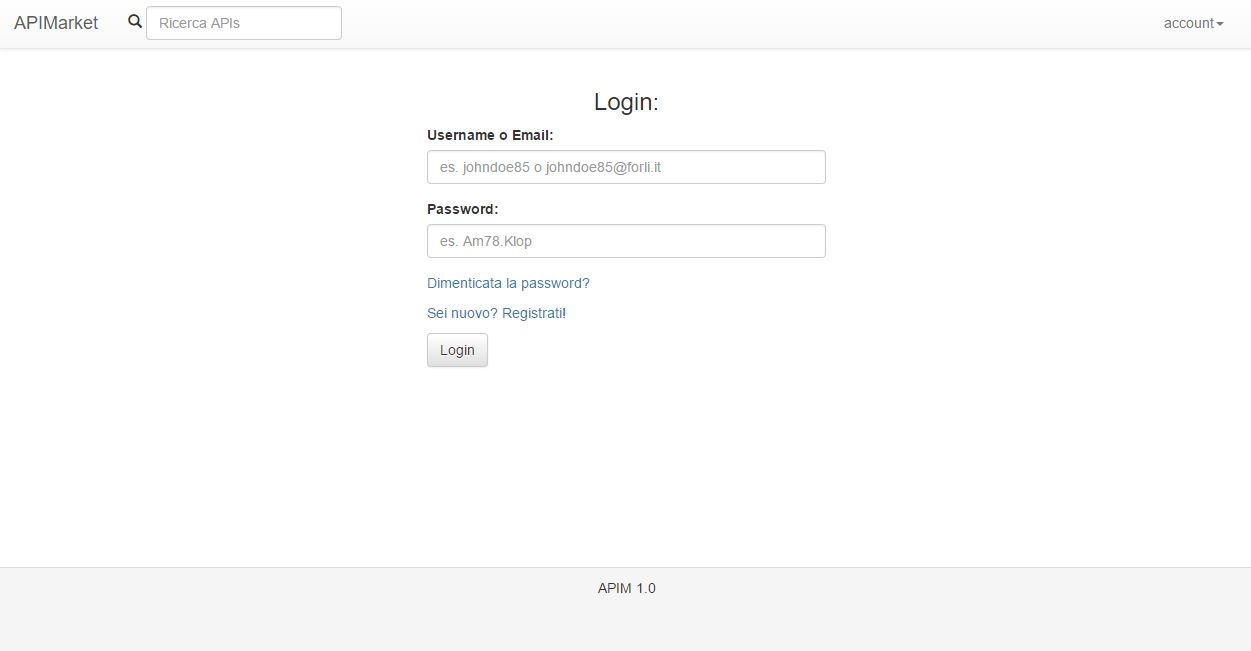
\includegraphics[scale=0.31]{img/APIM_login.JPG}}
		\caption{Login}
	\end{figure}
	
	\subsection{Conferma Login}
	Dopo aver inserito i dati di login e cliccato sul pulsante "Login", se i dati di accesso sono corretti, l'utente visualizza una pagina di conferma login, con la possibilità di recarsi sulla Homepage oppure nella gestione del proprio profilo.
	
	\label{Conferma Login}
	\begin{figure}[H]
		\centering
		\fbox{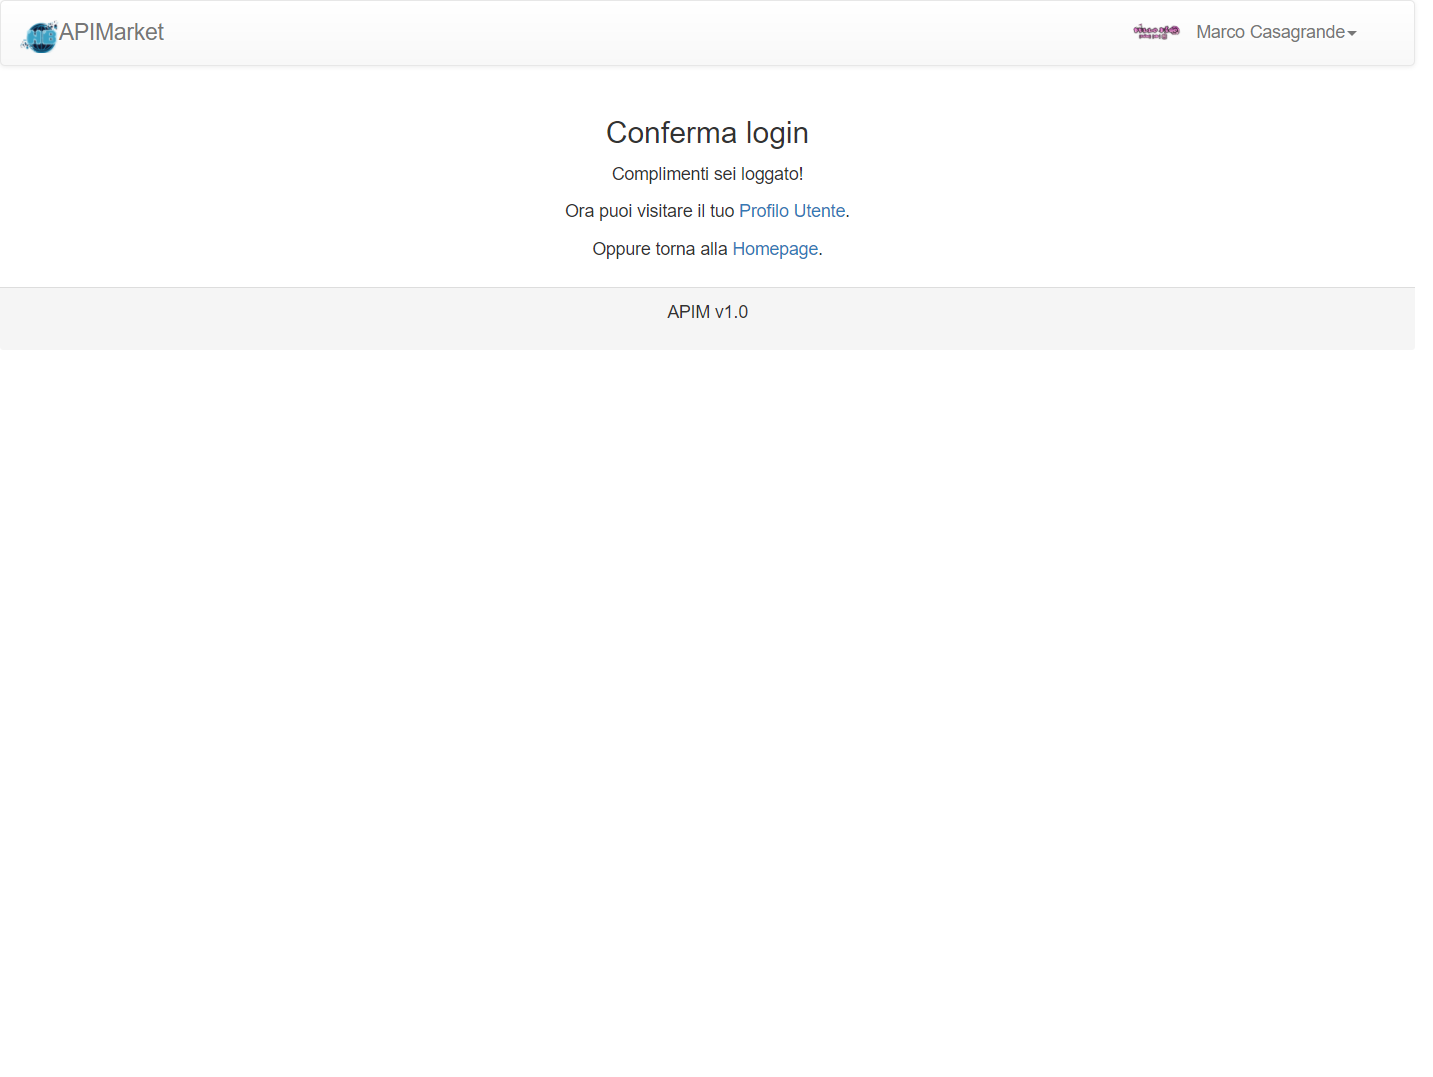
\includegraphics[scale=0.31]{img/APIM_confermaLogin.jpg}}
		\caption{Login}
	\end{figure}
	
	
	
	\subsection{Recupero Password}
	Qualora si fosse dimenticata la password, dalla schermata di login si può accedere alla pagina per il recupero della password. Inserendo l'indirizzo email si può ottenere un link per reimpostare i propri dati personali tramite una pagina dedicata. 
	
	\label{Recupero Password}
	\begin{figure}[H]
		\centering
		\fbox{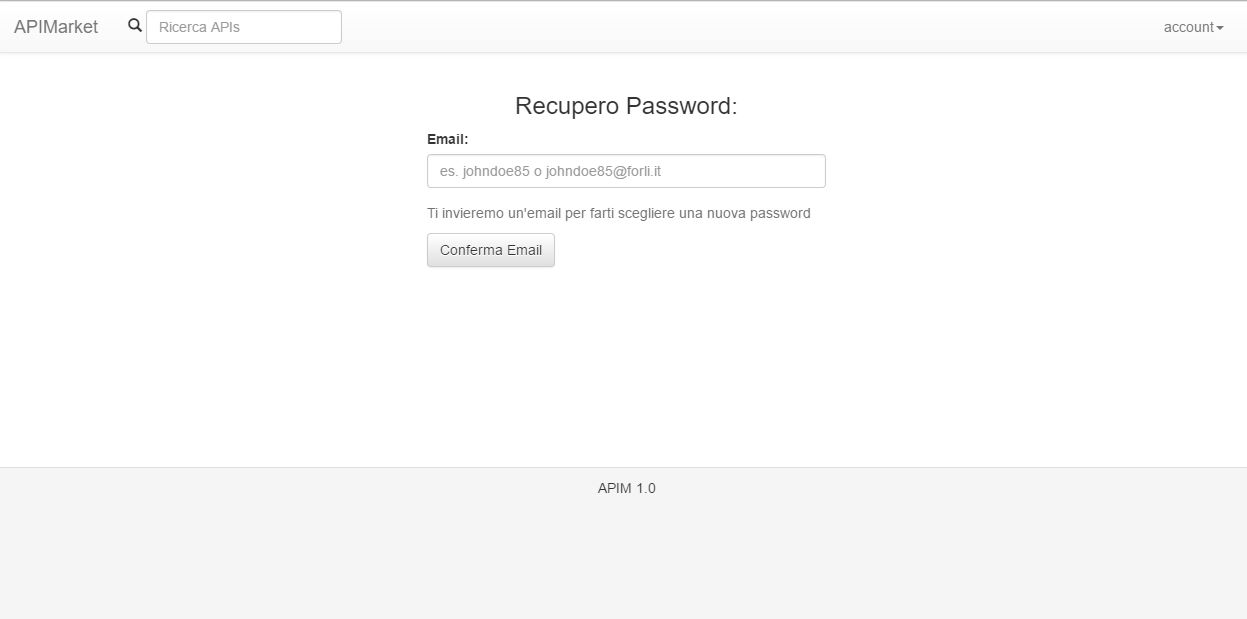
\includegraphics[scale=0.31]{img/APIM_recuperoPSW.JPG}}
		\caption{Recupero Password}
	\end{figure}

\subsection{Ricerca e visualizzazione API}

\subsubsection{Ricerca}
La funzionalità di ricerca è disponibile per qualsiasi categoria di utente. Essa permette, in base ad una parola chiave, di visualizzare le API relative contenute nella piattaforma. In seguito a ricerca, effettuata scrivendo sull'apposita barra la parola chiave desiderata, si può accedere ad un elenco dei risultati come mostrato. 

\label{Risultati ricerca}
\begin{figure}[H]
	\centering
	\fbox{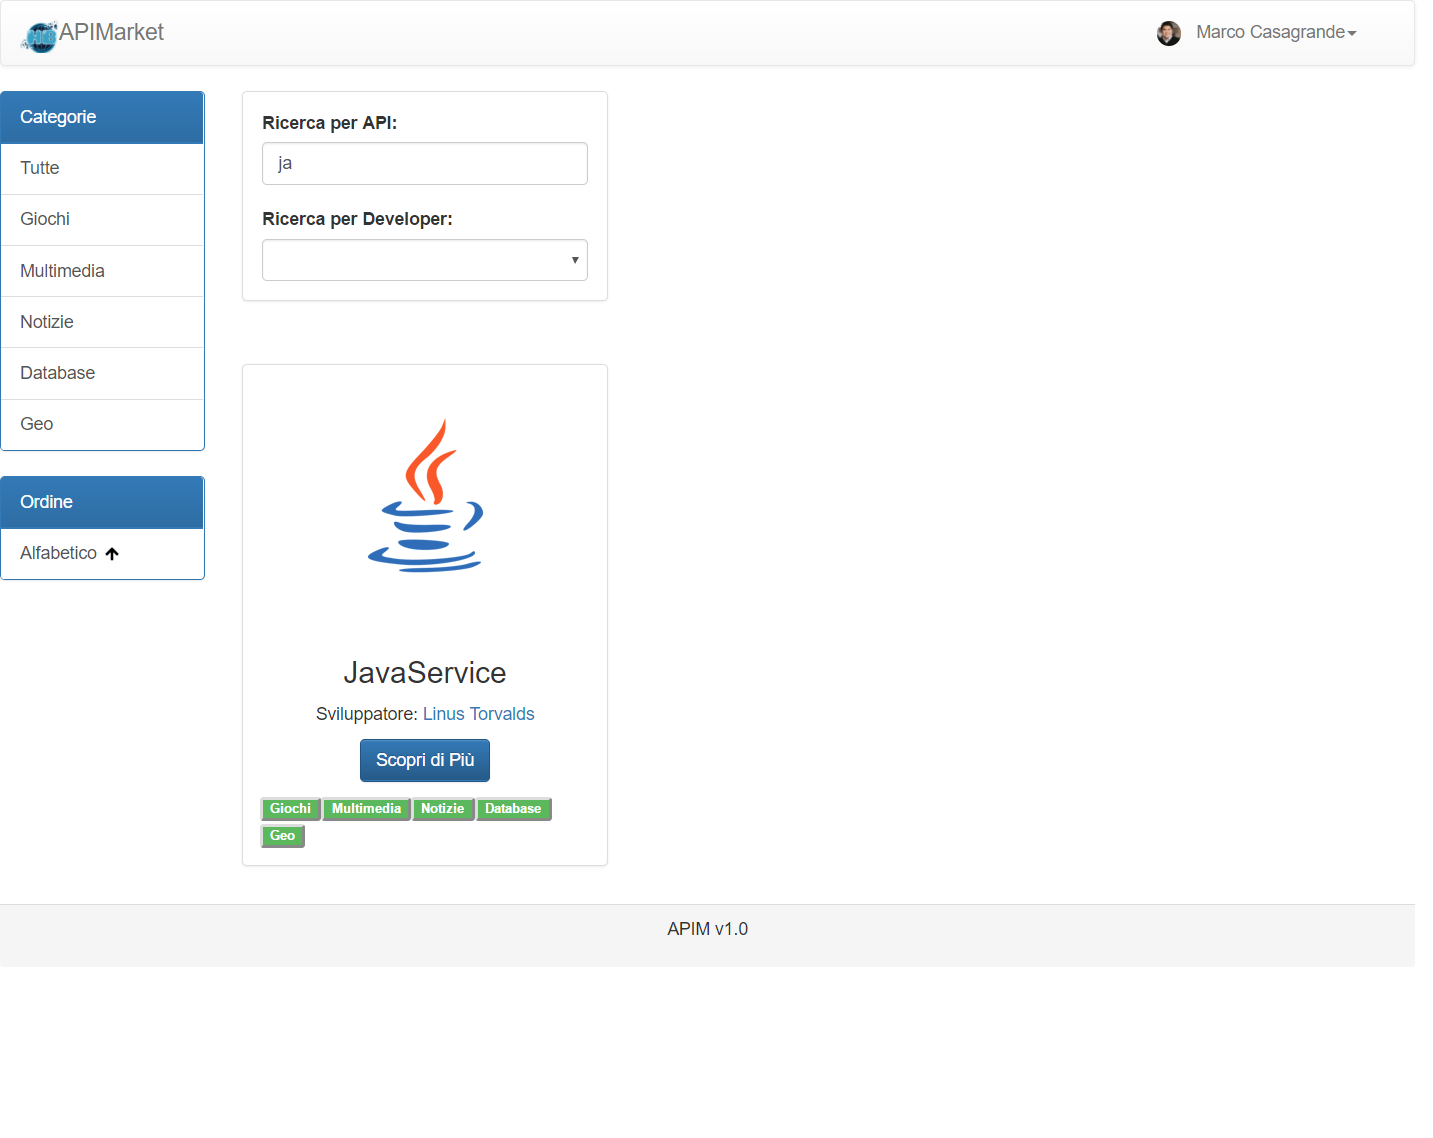
\includegraphics[scale=0.31]{img/APIM_ricerca.JPG}}
	\caption{Risultati ricerca}
\end{figure}


\subsubsection{Visualizzazione dettagli API}
Selezionando un API dall'elenco dei risultati, è possibile visualizzare i dati nel dettaglio, con relative specifiche. 


\label{Visualizzazione API}
\begin{figure}[H]
	\centering
	\fbox{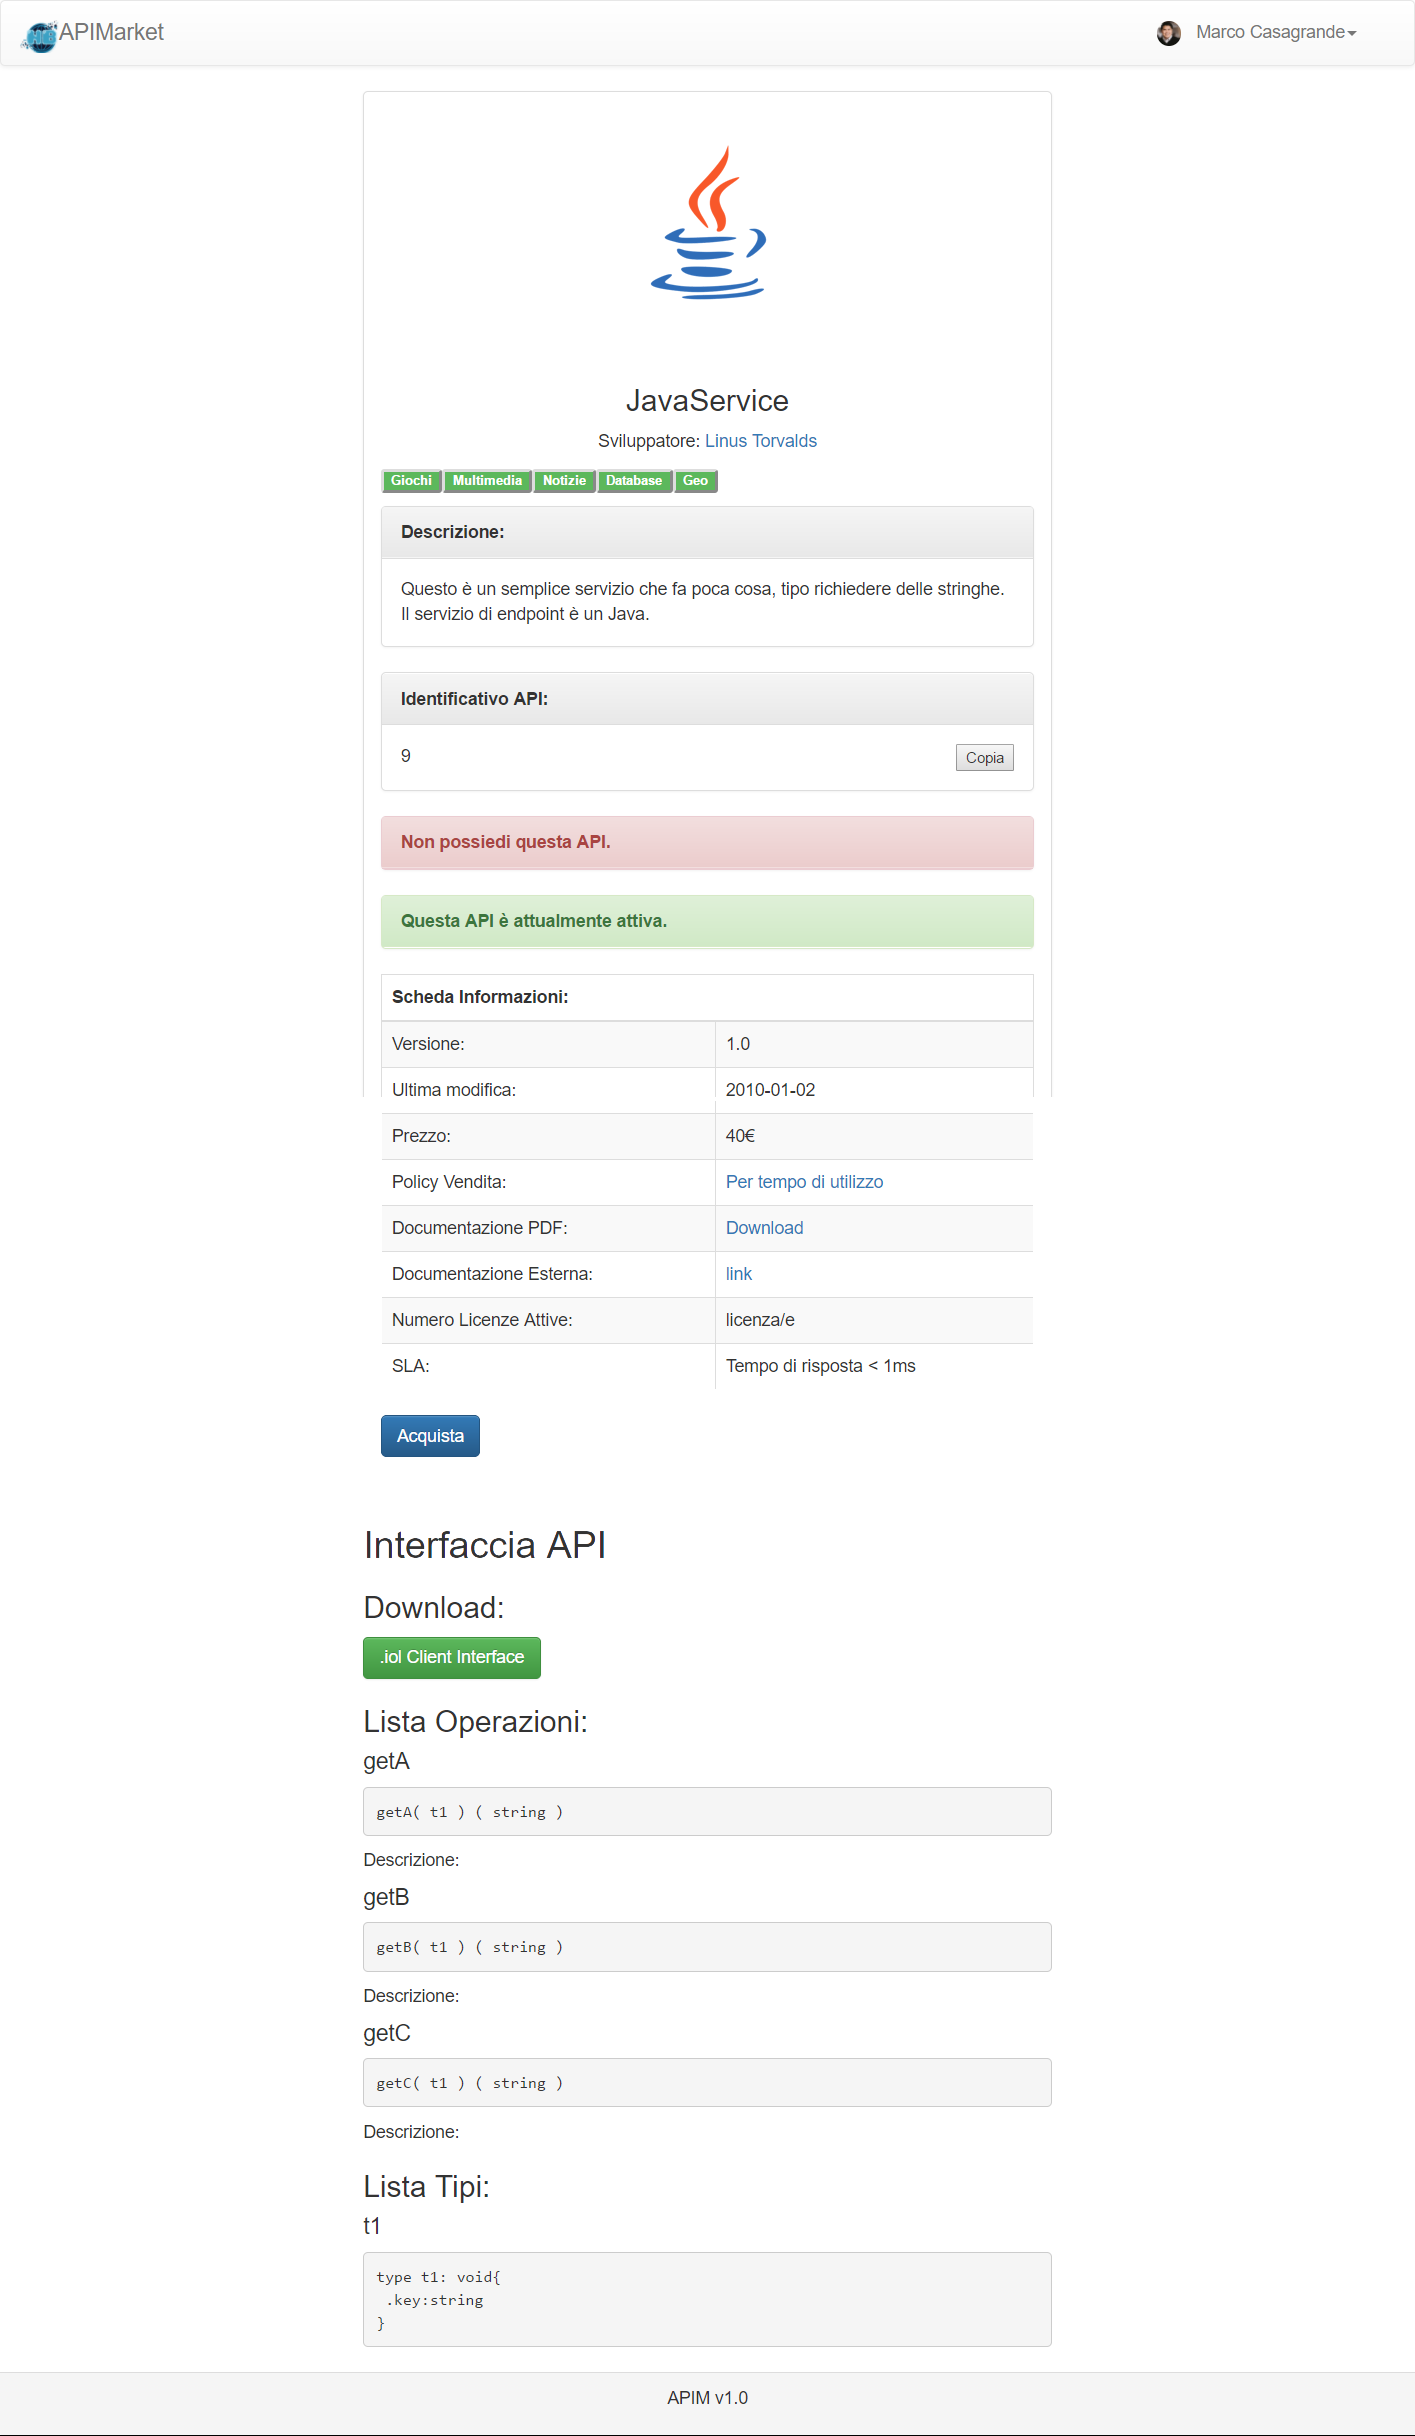
\includegraphics[scale=0.28]{img/APIM_dettagliApi.png}}
	\caption{Visualizzazione API}
\end{figure}

Ciascuna API presente nella piattaforma è caratterizzata da una policy di vendita, descritta all'interno di ciascun prodotto. E' possibile visualizzare i dettagli della policy clickando sull'apposito link nella schermata.

\label{Visualizza policy API}
\begin{figure}[H]
	\centering
	\fbox{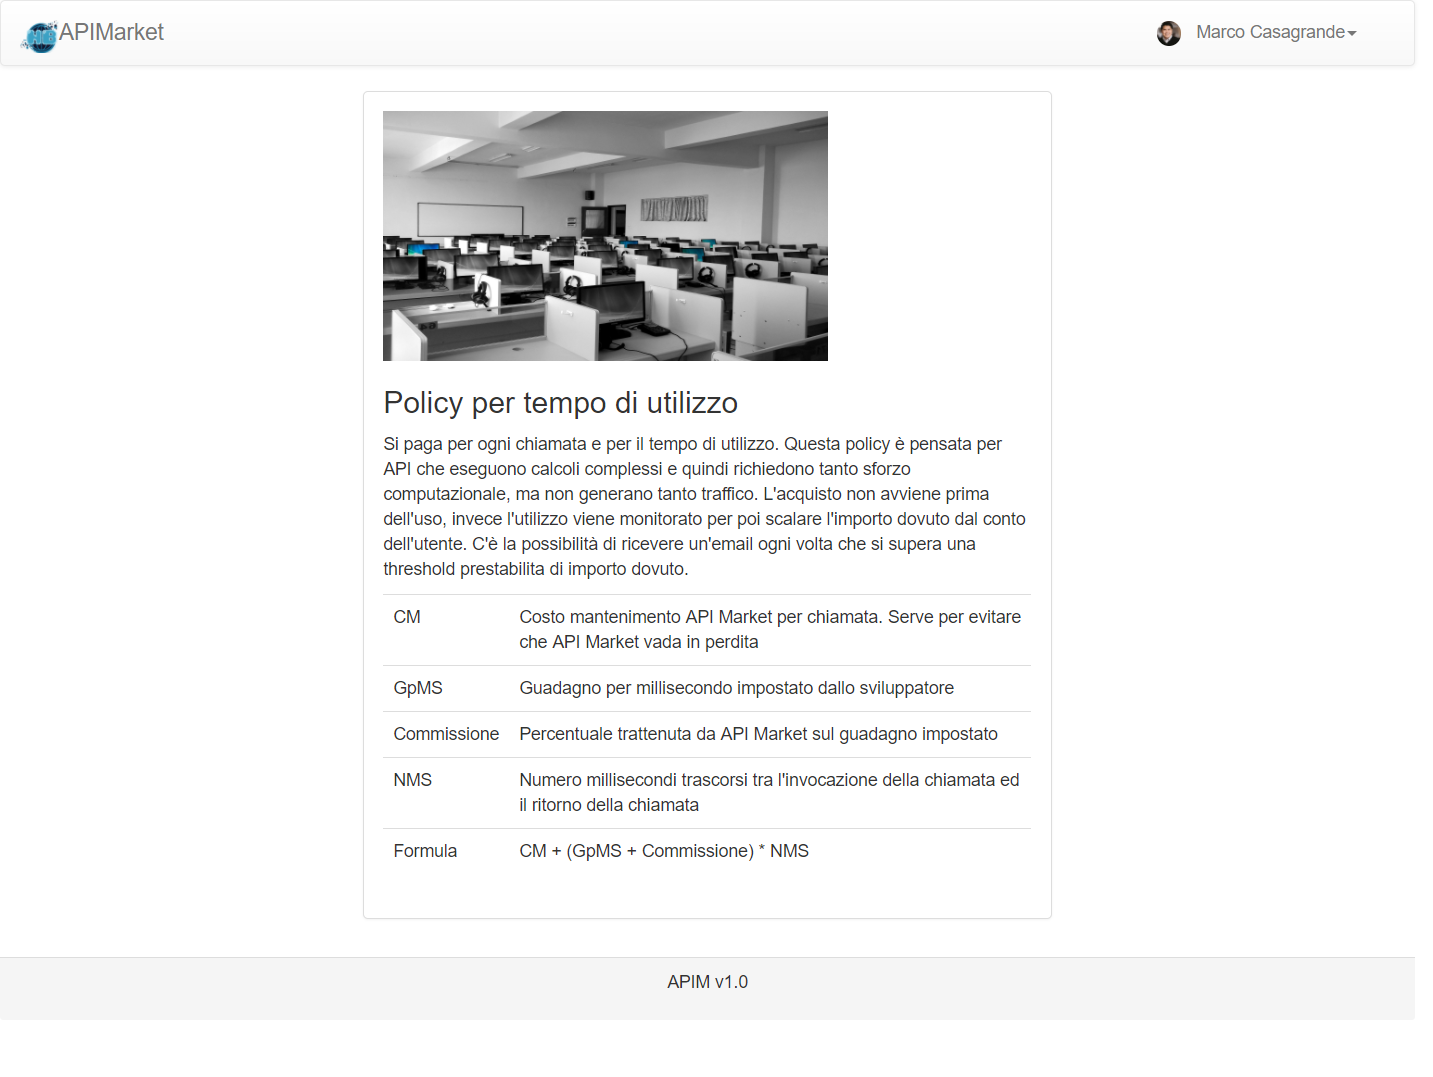
\includegraphics[scale=0.31]{img/APIM_policy.JPG}}
	\caption{Visualizza policy API}
\end{figure}

\subsubsection{Acquisto}
Qualora si decidesse di effettuare l'acquisto, nella schermata è presente un pulsante Acquista. Nella stessa schermata un utente loggato può inserire la quantità che intende acquistare, altrimenti chiederà di effettuare il login o la registrazione. Per maggiori relativi all'acquisto, si rimanda alla sezione 4.2 del presente manuale.




